\documentclass[11pt,a4paper]{article}

\usepackage[margin=1in]{geometry}
\usepackage[T1]{fontenc}
\usepackage[utf8]{inputenc}
\usepackage{lmodern}
\usepackage{amsmath,amssymb}
\usepackage{booktabs}
\usepackage{array}
\usepackage{longtable}
\usepackage{hyperref}
\usepackage{enumitem}
\usepackage{tikz}
\usetikzlibrary{arrows.meta,positioning,shapes.geometric}

\title{Movie Recommendation System: End-to-End Flow and Model Details}
\author{Project Documentation}
\date{\today}

\begin{document}
\maketitle
\tableofcontents
\newpage

\section{Project Overview}
This project implements a hybrid movie recommendation platform with:
\begin{itemize}[leftmargin=1.5em]
    \item Offline feature engineering from MovieLens-style data.
    \item Multiple recommenders: content-based, collaborative, hybrid, new-user, existing-user.
    \item Context adaptation by mood and time of day.
    \item Real-time user history updates from interface clicks.
    \item Human-readable explanation generation for each recommendation.
\end{itemize}

\section{End-to-End Flow}
\subsection{System Flow (High Level)}
\begin{center}
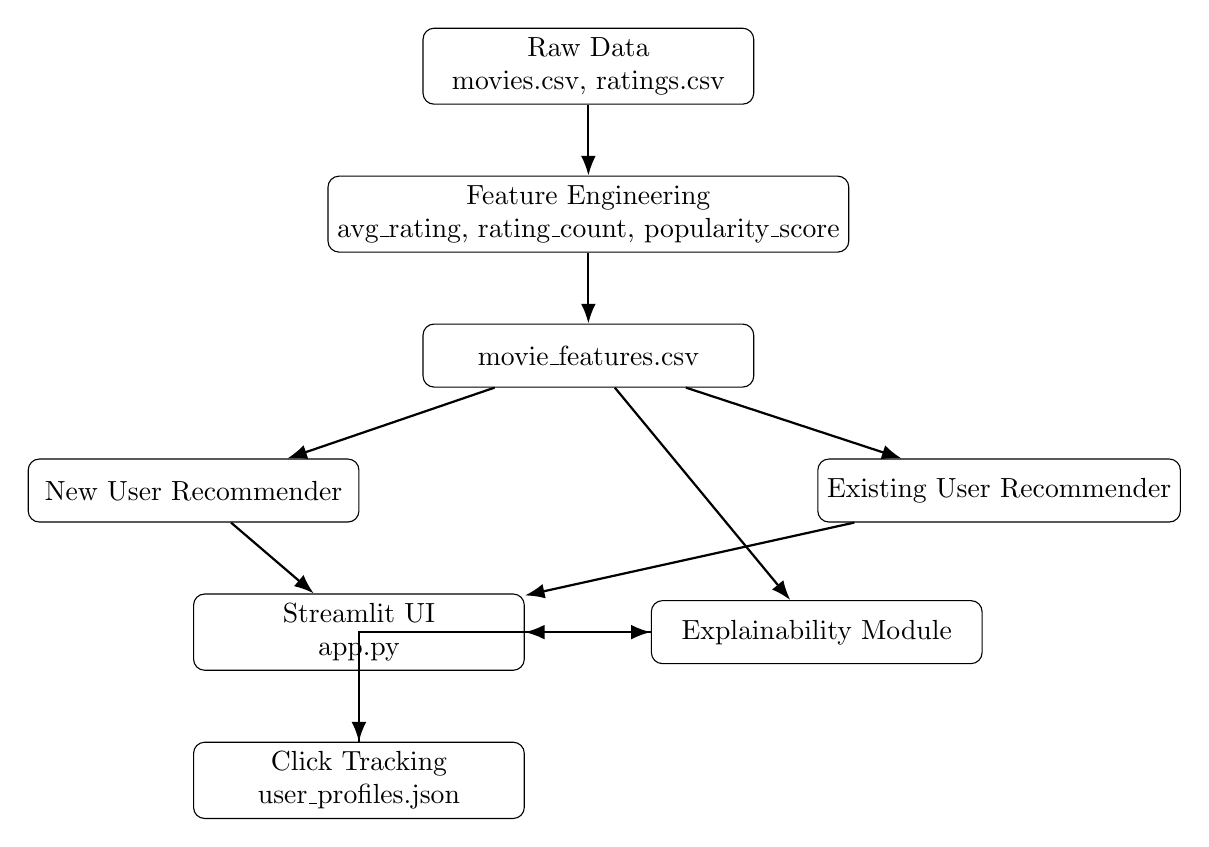
\begin{tikzpicture}[
    node distance=9mm and 8mm,
    box/.style={rectangle, rounded corners, draw, align=center, minimum width=4.2cm, minimum height=8mm},
    line/.style={-{Latex[length=2.5mm]}, thick}
]
\node[box] (raw) {Raw Data\\movies.csv, ratings.csv};
\node[box, below=of raw] (fe) {Feature Engineering\\avg\_rating, rating\_count, popularity\_score};
\node[box, below=of fe] (mf) {movie\_features.csv};
\node[box, below left=of mf] (new) {New User Recommender};
\node[box, below right=of mf] (exist) {Existing User Recommender};
\node[box, below=of new, xshift=2.1cm] (ui) {Streamlit UI\\app.py};
\node[box, below=of ui] (upd) {Click Tracking\\user\_profiles.json};
\node[box, right=16mm of ui] (exp) {Explainability Module};

\draw[line] (raw) -- (fe);
\draw[line] (fe) -- (mf);
\draw[line] (mf) -- (new);
\draw[line] (mf) -- (exist);
\draw[line] (new) -- (ui);
\draw[line] (exist) -- (ui);
\draw[line] (ui) -- (upd);
\draw[line] (mf) -- (exp);
\draw[line] (upd) |- (exp);
\draw[line] (exp) -- (ui);
\end{tikzpicture}
\end{center}

\subsection{Runtime Flow in UI}
\begin{enumerate}[leftmargin=1.5em]
    \item Load cached movie features and initialize recommender objects.
    \item User selects mood and user type (new or existing).
    \item New user path: choose preferred genres and liked movies, then score all movies.
    \item Existing user path: read recent watch history and score all movies.
    \item Display top recommendations with score and explanation.
    \item On click of \texttt{Watch}, append movie to persistent history JSON.
\end{enumerate}

\section{Data and Feature Engineering}
\subsection{Inputs}
\begin{itemize}[leftmargin=1.5em]
    \item \texttt{data/raw/movies.csv}: movieId, title, genres.
    \item \texttt{data/raw/ratings.csv}: userId, movieId, rating.
\end{itemize}

\subsection{Engineered Features}
Implemented in \texttt{src/data\_processing/feature\_engineering.py}:
\begin{align}
\text{avg\_rating}(m) &= \frac{1}{N_m}\sum_{i=1}^{N_m} r_{i,m} \\
\text{rating\_count}(m) &= N_m \\
\text{popularity\_score}(m) &= \text{avg\_rating}(m) \cdot \log(1 + \text{rating\_count}(m))
\end{align}
where $N_m$ is number of ratings for movie $m$.

\subsection{Output}
\texttt{data/processed/movie\_features.csv} stores metadata and engineered statistics used by all models.

\section{Model Details}
\subsection{Content-Based Recommender}
File: \texttt{src/models/content\_based.py}

\paragraph{Representation}
For each movie, a combined text field is built:
\begin{equation}
\text{combined}(m) = \text{title}(m) ~\Vert~ \text{genres}(m)
\end{equation}
TF-IDF vectorization converts text into sparse vector $\mathbf{v}_m$.

\paragraph{Similarity}
For a seed movie $s$, score each movie $m$ with cosine similarity (implemented using linear kernel on normalized TF-IDF):
\begin{equation}
\text{score}_{\text{content}}(s,m) = \cos(\mathbf{v}_s, \mathbf{v}_m)
\end{equation}
Top-$N$ highest scores are returned after excluding the seed movie itself.

\subsection{Collaborative Filtering Recommender}
File: \texttt{src/models/collaborative.py}

\paragraph{Algorithm}
Uses matrix factorization via Surprise SVD:
\begin{itemize}[leftmargin=1.5em]
    \item \texttt{n\_factors = 50}
    \item \texttt{n\_epochs = 10}
\end{itemize}

\paragraph{Training Optimizations in Code}
\begin{itemize}[leftmargin=1.5em]
    \item Randomly samples up to 300000 ratings for faster training.
    \item Retains active users only (more than 20 ratings).
\end{itemize}

\paragraph{Prediction}
For user $u$ and candidate movie $m$, model predicts:
\begin{equation}
\hat r_{u,m} = \mu + b_u + b_m + \mathbf{p}_u^T \mathbf{q}_m
\end{equation}
Top-$N$ movies by $\hat r_{u,m}$ are recommended from unrated candidate set (sampled up to 5000 movies for speed).

\subsection{Hybrid Recommender}
File: \texttt{src/models/hybrid.py}

\paragraph{Inputs}
\begin{itemize}[leftmargin=1.5em]
    \item Content model scores for top 50 movies from a seed movie.
    \item Collaborative predictions for top 50 movies for a user.
\end{itemize}

\paragraph{Normalization}
Both scores are min-max scaled to $[0,1]$:
\begin{equation}
\tilde x = \frac{x - x_{\min}}{x_{\max} - x_{\min}}
\end{equation}

\paragraph{Fusion}
Final score with blend parameter $\alpha$:
\begin{equation}
\text{final\_score}(m) = \alpha \cdot \tilde s_{\text{content}}(m) + (1-\alpha) \cdot \tilde s_{\text{collab}}(m)
\end{equation}
Default is $\alpha = 0.5$.

\subsection{Context Boost Module}
File: \texttt{src/models/context\_model.py}

Context adds bonus based on mood and time-of-day genre rules:
\begin{equation}
\text{final\_score}'(m) = \text{final\_score}(m) + \text{context\_bonus}(m)
\end{equation}

\paragraph{Mood bonus examples}
\begin{itemize}[leftmargin=1.5em]
    \item happy $\rightarrow$ Comedy gets +0.2
    \item serious $\rightarrow$ Drama gets +0.2
    \item excited $\rightarrow$ Action gets +0.2
\end{itemize}

\paragraph{Time bonus}
\begin{itemize}[leftmargin=1.5em]
    \item night $\rightarrow$ Thriller/Horror gets +0.2
\end{itemize}

\subsection{New User Recommender (Cold Start)}
File: \texttt{src/models/new\_user\_recommender.py}

For each candidate movie $m$:
\begin{equation}
\text{score}(m)=0.4\cdot G(m)+0.3\cdot L(m)+0.2\cdot P(m)+0.1\cdot M(m)
\end{equation}
where:
\begin{itemize}[leftmargin=1.5em]
    \item $G(m)$: fraction of preferred genres matched.
    \item $L(m)$: maximum TF-IDF similarity to any liked movie.
    \item $P(m)$: popularity score from feature table.
    \item $M(m)$: mood match indicator (0 or 1).
\end{itemize}

Liked movies are excluded from output.

\paragraph{Diversity Penalty}
After taking top 100 by raw score, each movie receives penalty by repeated genres already seen in ranked traversal:
\begin{equation}
\text{adjusted\_score}(m)=\text{score}(m)-0.05\cdot \text{penalty}(m)
\end{equation}
Then greedy selection builds a more genre-diverse top-$N$.

\subsection{Existing User Recommender}
File: \texttt{src/models/existing\_user\_recommender.py}

\paragraph{User Preference Extraction}
From recent watch history, top 3 most frequent genres are extracted.

\paragraph{Scoring}
For movie $m$:
\begin{equation}
\text{score}(m)=0.35\cdot S(m)+0.25\cdot G(m)+0.25\cdot P(m)
\end{equation}
where:
\begin{itemize}[leftmargin=1.5em]
    \item $S(m)$: max TF-IDF similarity to any recent movie.
    \item $G(m)$: genre match indicator against extracted preferred genres.
    \item $P(m)$: popularity score.
\end{itemize}
Recent movies are excluded, and the same diversity-penalty strategy as new-user model is applied.

\paragraph{Implementation Note}
Current weights sum to $0.85$ (not $1.0$). Ranking still works because scaling is monotonic, but normalization of weights may improve interpretability.

\section{Explainability Module}
File: \texttt{src/explainability/explain.py}

Explanation rules are generated in this order:
\begin{enumerate}[leftmargin=1.5em]
    \item Must-watch override: if movie is popular and outside preferred genres, return ``Must Watch'' message.
    \item History-based reason: similar genre to user's last watched movie.
    \item Mood-based reason: genre aligns with selected mood map.
    \item Fallback reason: belongs to main genre.
\end{enumerate}

Final sentence format:
\begin{equation}
\texttt{"Recommended because it "} + \texttt{reasons joined by commas} + \texttt{"."}
\end{equation}

\section{Real-Time Update and User Profile Persistence}
File: \texttt{src/realtime/update\_model.py}

\begin{itemize}[leftmargin=1.5em]
    \item User profiles are stored in \texttt{data/processed/user\_profiles.json}.
    \item \texttt{add\_clicked\_movie} appends selected movie, removes duplicates while preserving latest order, and keeps only last 5 entries.
    \item \texttt{get\_recent\_history} feeds existing-user recommendation logic.
\end{itemize}

This creates an online feedback loop: interactions immediately influence future recommendations.

\section{Serving Layer}
\subsection{Streamlit Application}
File: \texttt{app.py}

\begin{itemize}[leftmargin=1.5em]
    \item Uses \texttt{st.cache\_data} for feature table.
    \item Uses \texttt{st.cache\_resource} for model objects.
    \item Branches between new-user and existing-user recommendation flows.
    \item Displays ranked list with model score and generated explanation.
    \item Tracks clicks to update persistent watch history.
\end{itemize}

\subsection{CLI Entry}
File: \texttt{main.py}

Provides terminal-based interaction for recommendation and click simulation.

\section{Complexity and Practical Notes}
\begin{itemize}[leftmargin=1.5em]
    \item TF-IDF fit is linear in corpus size and vocabulary footprint.
    \item Pairwise similarity is computed query-vs-all (efficient for single seed).
    \item Collaborative model limits data and candidate pools for speed.
    \item Diversity post-processing is greedy and lightweight for top candidates.
\end{itemize}

\section{How to Compile}
From project root:
\begin{verbatim}
pdflatex project_flow_and_models.tex
\end{verbatim}
Run twice if table of contents links need full resolution.

\end{document}
